\documentclass[12pt, a4paper]{article}
\usepackage{../../../myconfig} % Gọi file cấu hình từ ngoài gốc vào

% ==========================================
% BẮT ĐẦU NỘI DUNG TÀI LIỆU
% ==========================================
\begin{document}

% Truyền 3 tham số: {Nhãn cam} {Chữ to chính giữa} {Chữ ở góc phải Header}
\titlebox{KTDK}{Đề kiểm tra định kỳ lần 7}{Kiểm tra định kỳ}

\textit{\textbf{Phần I: Thí sinh trả lời từ câu 1 đến câu 12, mỗi câu thí sinh chỉ chọn một phương án}}

\vspace{0.5cm}

% --- CÂU 1 ---
\questionLinesManual{0}{1}{Cho \(\displaystyle\int_{2}^{5} f(x) dx = 2\) và \(\displaystyle\int_{2}^{5} g(x) dx = 5\). Giá trị của tích phân \(\displaystyle\int_{2}^{5} [f(x) - 2g(x)] dx\) bằng}{%
    \begin{tasks}(4)
        \task \(-8\)
        \task \(12\)
        \task \(1\)
        \task \(-3\)
    \end{tasks}
}

% --- CÂU 2 ---
\questionLinesManual{0}{2}{Gọi \(V\) là thể tích khối tròn xoay tạo thành khi quay hình phẳng giới hạn bởi đồ thị hàm số \(y = e^x\), trục hoành và hai đường thẳng \(x = 0, x = 3\) quanh trục \(Ox\). Khi đó \(V\) bằng}{%
    \begin{tasks}(4)
        \task \(\pi \displaystyle\int_{0}^{3} e^{2x} dx\)
        \task \(\displaystyle\int_{0}^{3} e^{2x} dx\)
        \task \(\displaystyle\int_{0}^{3} e^x dx\)
        \task \(\pi \displaystyle\int_{0}^{3} e^x dx\)
    \end{tasks}
}

% --- CÂU 3 ---
\questionLinesManual{0}{3}{Nguyên hàm của hàm số \(f(x) = \sin 2x\) là:}{%
    \begin{tasks}(4)
        \task \(\dfrac{1}{2}\cos x + C\)
        \task \(-\dfrac{1}{2}\cos 2x + C\)
        \task \(\dfrac{1}{2}\cos 2x + C\)
        \task \(-\dfrac{1}{2}\cos x + C\)
    \end{tasks}
}

% --- CÂU 4 ---
\questionLinesManual{0}{4}{Tìm tất cả nguyên hàm \(F(x)\) của hàm số \(f(x) = x - \dfrac{1}{x}\).}{%
    \begin{tasks}(2)
        \task \(F(x) = \dfrac{1}{2}x^2 - \ln|x| + C\)
        \task \(F(x) = 1 - \ln|x| + C\)
        \task \(F(x) = \dfrac{1}{2}x^2 - \ln|x|\)
        \task \(F(x) = \dfrac{1}{2}x^2 - \ln x + C\)
    \end{tasks}
}

% --- CÂU 5 ---
\questionLinesManual{0}{5}{Cho vật thể giới hạn bởi hai mặt phẳng có phương trình \(x = 0\) và \(x = 2\). Cắt phần vật thể này bởi mặt phẳng vuông góc với trục \(Ox\) tại điểm có hoành độ \(x\) (\(0 \leq x \leq 2\)) thì phần chung của mặt phẳng và vật thể là một tam giác đều có độ dài cạnh bằng \(x^2\sqrt{2-x}\). Tính thể tích của vật thể này.}{%
    \begin{tasks}(4)
        \task \(V = \dfrac{8\sqrt{3}}{15}\)
        \task \(V = \dfrac{4\sqrt{3}}{15}\)
        \task \(V = \dfrac{16}{15}\)
        \task \(V = \dfrac{32}{15}\)
    \end{tasks}
}

% --- CÂU 6 ---
\questionLinesManual{0}{6}{Gọi \(S\) là diện tích hình phẳng giới hạn bởi các đường \(y = f(x)\), trục hoành và hai đường thẳng \(x = -3\), \(x = 2\), như hình vẽ bên dưới. Đặt \(a = \displaystyle\int_{-3}^{1} f(x) dx\), \(b = \displaystyle\int_{1}^{2} f(x) dx\). Mệnh đề nào sau đây là đúng?

\begin{center}
\begin{tikzpicture}[scale=1.1, >=stealth]
    % 1. Tô miền gạch sọc (Hatching) với khoảng cách gạch dày dặn, đẹp mắt
    % Miền S1: từ x = -3 đến x = 1 (bên dưới trục hoành)
    \pattern[pattern=north east lines, pattern color=black!60] 
        (-3,0) -- plot[domain=-3:1, samples=100] (\x, {2^(\x-1)-1}) -- (1,0) -- cycle;

    % Miền S2: từ x = 1 đến x = 2 (bên trên trục hoành)
    \pattern[pattern=north east lines, pattern color=black!60] 
        (1,0) -- plot[domain=1:2, samples=100] (\x, {2^(\x-1)-1}) -- (2,0) -- cycle;
    % 3. Trục tọa độ Ox, Oy
    \draw[->, thick] (-4.0, 0) -- (3.2, 0) node[above, font=\small] {$x$};
    \draw[->, thick] (0, -1.5) -- (0, 1.8) node[left, font=\small] {$y$};
    \node[above left, font=\small] at (0, 0) {$0$};

    % 4. Đồ thị hàm số y = f(x) với độ cong vừa phải, không bị kéo quá dài

    \draw[thick, domain=-3:2, samples=100] 
        plot (\x, {2^(\x-1)-1});

    % 5. Đánh dấu các điểm và số trên trục
    \fill (-3, 0) circle (1.2pt) node[above, font=\small, yshift=2pt] {$-3$};
    \fill (1, 0)  circle (1.2pt) node[above left, font=\small] {$1$};
    \fill (2, 0)  circle (1.2pt) node[below, font=\small, yshift=-2pt] {$2$};

\end{tikzpicture}
\end{center}
}{%
    \begin{tasks}(4)
        \task \(S = -a - b\)
        \task \(S = a + b\)
        \task \(S = b - a\)
        \task \(S = a - b\)
    \end{tasks}
}

% --- CÂU 7 ---
\questionLinesManual{0}{7}{Hàm số nào sau đây không là một nguyên hàm của hàm số \(f(x) = 3x^2 + 2x - 1\)?}{%
    \begin{tasks}(2)
        \task \(F(x) = x^3 + x^2 - x\)
        \task \(F(x) = x^3 + x^2 - x + 2026\)
        \task \(F(x) = x^3 + x^2 - 1\)
        \task \(F(x) = x^3 + x^2 - x - 1\)
    \end{tasks}
}

% --- CÂU 8 ---
\questionLinesManual{0}{8}{Cho hàm số \(f(x) = x^2 - \dfrac{4}{x}\). Giá trị của \(\displaystyle\int_{1}^{2} f'(x) dx\) bằng}{%
    \begin{tasks}(4)
        \task \(5 - \ln 2\)
        \task \(\dfrac{7}{3} - \ln 2\)
        \task \(5\)
        \task \(\dfrac{7}{3}\)
    \end{tasks}
}

% --- CÂU 9 ---
\questionLinesManual{0}{9}{Giá trị của \(P = \displaystyle\int_{-1}^{2} \dfrac{2x^2 - 5x - 2}{x - 3} dx\) là}{%
    \begin{tasks}(4)
        \task \(P = -6 + \ln 4\)
        \task \(P = 6 - \ln 4\)
        \task \(P = 3 + \ln 5\)
        \task \(P = 3 - \ln 5\)
    \end{tasks}
}

% --- CÂU 10 ---
\questionLinesManual{0}{10}{Cho hình phẳng \((H)\) giới hạn bởi đồ thị các hàm số \(y = 2e^x\), trục tung, trục hoành và đường thẳng \(x = 1\). Diện tích của hình \((H)\) là}{%
    \begin{tasks}(4)
        \task \(2e - 2\)
        \task \(2e - 1\)
        \task \(2e + 2\)
        \task \(2e + 1\)
    \end{tasks}
}

% --- CÂU 11 ---
\questionLinesManual{0}{11}{Biết \(I = \displaystyle\int_{1}^{2} \dfrac{1}{2x^2 + 5x + 3} dx = \ln\dfrac{a}{b}\) với \(a, b\) là các số lớn hơn 1, phân số \(\dfrac{a}{b}\) tối giản. Giá trị \(T = a + b\) bằng}{%
    \begin{tasks}(4)
        \task 28
        \task 29
        \task 12
        \task 10
    \end{tasks}
}

% --- CÂU 12 ---
\questionLinesManual{0}{12}{Cho hàm số \(y = f(x)\) liên tục trên \(\mathbb{R}\), thỏa mãn \(\displaystyle\int_{17}^{2026} f(x) dx = 8\) và \(\displaystyle\int_{89}^{2026} f(x) dx = 10\). Giá trị của biểu thức \(\displaystyle\int_{17}^{89} f(x) dx\) bằng:}{%
    \begin{tasks}(4)
        \task 18
        \task 2026
        \task 2
        \task -2
    \end{tasks}
}
\newpage

\textit{\textbf{Phần II: Thí sinh trả lời từ câu 13 đến câu 16; trong mỗi ý a), b), c), d) ở mỗi câu, thí sinh chọn đúng hoặc sai.}}

\vspace{0.3cm}

% --- CÂU 13 ---
\questionTrueFalse{0}{13}{Một cây cà chua khi mới trồng có chiều cao 15cm. Gọi \(h(t)\) là chiều cao của cây cà chua tại thời điểm đúng \(t\) tuần sau khi trồng (đơn vị: cm, \(0 \leq t \leq 16\)). Biết rằng tốc độ tăng chiều cao của cây cà chua đó được cho bởi hàm số \(h'(t) = -0,02t^3 + 0,32t^2\) (đơn vị: cm/tuần).}{
    \textbf{a)} & Tại thời điểm đúng \(t\) tuần sau khi trồng, chiều cao của cây cà chua là \(h(t) = -\dfrac{t^4}{200} + \dfrac{32t^3}{300}\) (cm).
    & \textcolor{amberorange}{$\bigcirc$} & \textcolor{amberorange}{$\bigcirc$} \\ \hline
    
    \textbf{b)} & Tại thời điểm tốc độ tăng chiều cao của cây cà chua lớn nhất, cây cà chua cao hơn 80 (cm).
    & \textcolor{amberorange}{$\bigcirc$} & \textcolor{amberorange}{$\bigcirc$} \\ \hline
    
    \textbf{c)} & Trong khoảng thời gian 10 tuần đầu kể từ khi trồng, tốc độ tăng chiều cao trung bình của cây cà chua lớn hơn 5,6 (cm/tuần).
    & \textcolor{amberorange}{$\bigcirc$} & \textcolor{amberorange}{$\bigcirc$} \\ \hline
    
    \textbf{d)} & Tại thời điểm đúng 6 tuần sau khi trồng, chiều cao của cây cà chua là 31,56 (cm).
    & \textcolor{amberorange}{$\bigcirc$} & \textcolor{amberorange}{$\bigcirc$} \\
}

% --- CÂU 14 ---
\questionTrueFalse{0}{14}{Một ô tô bắt đầu chuyển động thẳng nhanh dần đều với vận tốc \(v(t) = 5t\) (m/s), trong đó \(t\) là thời gian tính bằng giây kể từ khi ô tô bắt đầu chuyển động. Đi được 6(s) người lái xe phát hiện chướng ngại vật và phanh gấp, ô tô tiếp tục chuyển động chậm dần đều với gia tốc \(a = -5\) (m/s\(^2\)).}{
    \textbf{a)} & Tốc độ của ô tô tại thời điểm 10(s) tính từ lúc xuất phát là 10 (m/s).
    & \textcolor{amberorange}{$\bigcirc$} & \textcolor{amberorange}{$\bigcirc$} \\ \hline
    
    \textbf{b)} & Quãng đường ô tô chuyển động được trong 6 giây đầu tiên là 80 m.
    & \textcolor{amberorange}{$\bigcirc$} & \textcolor{amberorange}{$\bigcirc$} \\ \hline
    
    \textbf{c)} & Quãng đường \(S\), đơn vị: mét, mà ô tô chuyển động được kể từ lúc bắt đầu đạp phanh đến khi dừng lại được tính theo công thức \(S = \displaystyle\int_{0}^{6} (30 - 5t) dt\).
    & \textcolor{amberorange}{$\bigcirc$} & \textcolor{amberorange}{$\bigcirc$} \\ \hline
    
    \textbf{d)} & Quãng đường ô tô chuyển động được kể từ lúc bắt đầu chuyển động cho đến khi dừng lại là 170 m.
    & \textcolor{amberorange}{$\bigcirc$} & \textcolor{amberorange}{$\bigcirc$} \\
}

% --- CÂU 15 ---
\questionTrueFalse{0}{15}{Bút viết của một băng vẽ điện tử được để trong một chiếc giá là một khối tròn xoay có mặt cắt qua trục là một hình phẳng có hình dạng và các kích thước gắn với hệ trục tọa độ \(Oxy\) như hình vẽ.

\begin{figure}[H]
    \centering
    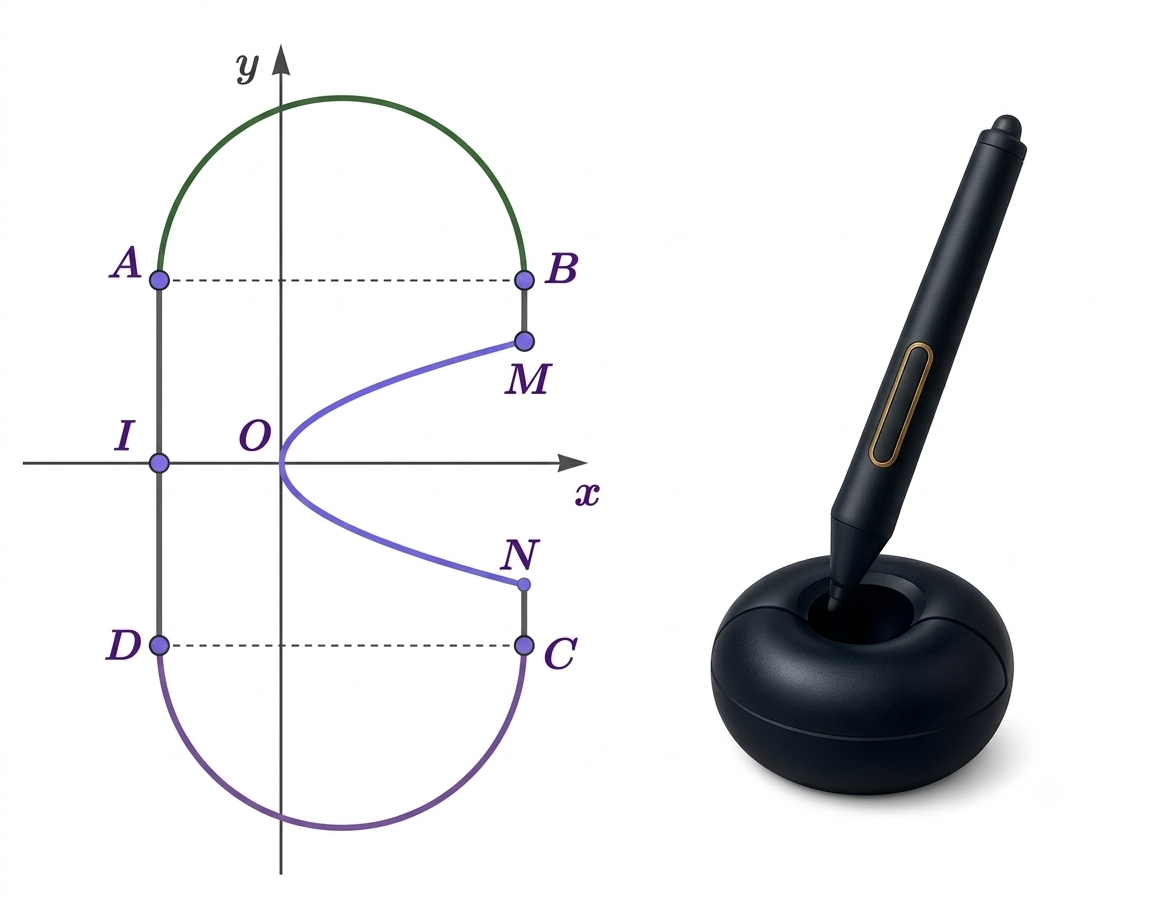
\includegraphics[width=0.7\textwidth]{images/Cau15.png}
\end{figure}

Biết biên của mặt cắt gồm hai nửa đường tròn đường kính \(AB, CD\) và một cung của parabol đỉnh \(O\), nhận \(Ox\) là trục đối xứng; cho \(AB = CD = 3\) cm, \(OI = 1\) cm, \(AD = 3\) cm, \(MN = 2\) cm, đơn vị trên hệ trục là cm.}{
    \textbf{a)} & Phương trình của parabol là \(y^2 = \dfrac{1}{2}x\).
    & \textcolor{amberorange}{$\bigcirc$} & \textcolor{amberorange}{$\bigcirc$} \\ \hline
    
    \textbf{b)} & Diện tích mặt cắt, làm tròn tới hàng đơn vị, là 14 cm\(^2\).
    & \textcolor{amberorange}{$\bigcirc$} & \textcolor{amberorange}{$\bigcirc$} \\ \hline
    
    \textbf{c)} & Thể tích phần lõm của giá để bút được tính bằng công thức \(\pi \displaystyle\int_{0}^{2} \dfrac{1}{2}x dx\).
    & \textcolor{amberorange}{$\bigcirc$} & \textcolor{amberorange}{$\bigcirc$} \\ \hline
    
    \textbf{d)} & Thể tích của toàn bộ giá để bút, làm tròn tới hàng phần chục, bằng 65,4 cm\(^3\).
    & \textcolor{amberorange}{$\bigcirc$} & \textcolor{amberorange}{$\bigcirc$} \\
}

\questionTrueFalse{0}{16}{Khối chỏm cầu có bán kính \( R = 10 \) và chiều cao \( h = 8 \) sinh ra khi quay hình phẳng giới hạn bởi cung tròn có phương trình \( y = \sqrt{100 - x^2} \), trục hoành và hai đường thẳng \( x = 2, x = 10 \) xung quanh trục \( Ox \).

\begin{center}
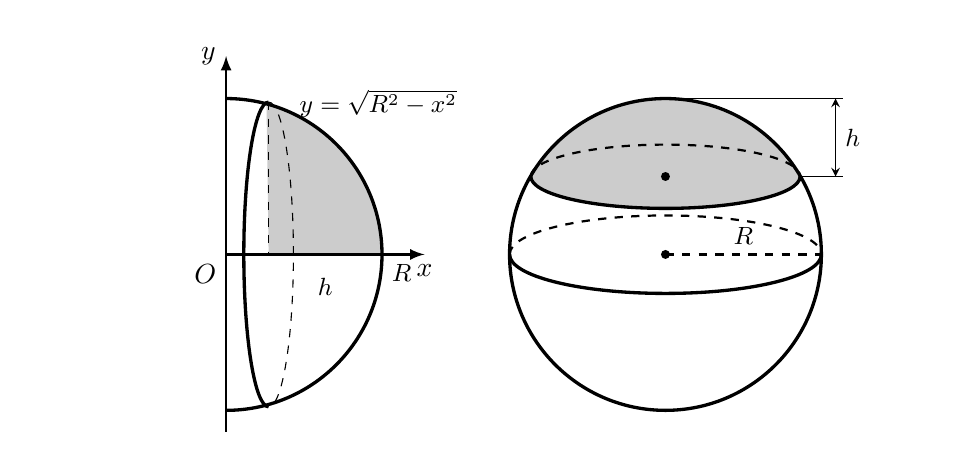
\begin{tikzpicture}[scale=0.9, >=latex]
    % Giới hạn vùng hiển thị bằng \clip
    \clip (-2.8, -2.7) rectangle (10.0, 3.2);

    % ==================== HÌNH 1: HỆ TRỤC Oxyz & CHỎM CẦU TRÒN XOAY ====================
    \begin{scope}[shift={(0,0)}]
        % 1. Tô màu phần chỏm cầu (miền xám)
        \fill[gray!40] (0.6, 0) -- (2.2, 0) 
            arc [start angle=0, end angle=75, radius=2.2] 
            -- cycle;

        % 2. Các trục tọa độ
        \draw[->, thick] (0, 0) -- (2.8, 0) node[below] {$x$};
        \draw[->, thick] (0, -2.5) -- (0, 2.8) node[left] {$y$};
        \node[below left] at (0, 0) {$O$};

        % 3. Cung tròn nửa cầu y = sqrt(R^2 - x^2)
        \draw[very thick] (0, 2.2) arc (90:-90:2.2);

        % 4. Mặt đáy chỏm cầu: Nửa sau NÉT ĐỨT, nửa trước NÉT LIỀN
        \draw[very thick] (0.6, 2.15) arc [start angle=90, end angle=270, x radius=0.35, y radius=2.15];
        \draw[dashed] (0.6, 2.15) arc [start angle=90, end angle=-90, x radius=0.35, y radius=2.15];
        \draw[dashed] (0.6, 2.15)-- (0.6,0);

        \node[below, font=\small] at (1.4, -0.2) {$h$};

        % Điểm R
        \node[below right, font=\small] at (2.2, 0) {$R$};

        % Nhãn phương trình
        \node[above right, font=\small] at (0.9, 1.8) {$y = \sqrt{R^2 - x^2}$};
    \end{scope}

    % ==================== HÌNH 2: KHỐI CẦU VÀ CHỎM CẦU ====================
    % Đã tăng khoảng cách x (shift={(6.2,0)}) để 2 hình xa nhau hơn
    \begin{scope}[shift={(6.2,0)}]
        % 1. Tô màu phần chỏm cầu bên trên
        \fill[gray!40] (0, 1.1) ellipse (1.9cm and 0.45cm);
        \fill[gray!40] (-1.9, 1.1) arc [start angle=150, end angle=30, radius=2.2] -- cycle;

        % 2. Mặt cầu bên ngoài
        \draw[very thick] (0,0) circle (2.2cm);

        % 3. Đường xích đạo: Nửa sau NÉT ĐỨT, nửa trước NÉT LIỀN
        \draw[thick, dashed] (-2.2, 0) arc [start angle=180, end angle=0, x radius=2.2, y radius=0.55];
        \draw[very thick] (-2.2, 0) arc [start angle=180, end angle=360, x radius=2.2, y radius=0.55];

        % 4. Đáy chỏm cầu: Nửa sau NÉT ĐỨT, nửa trước NÉT LIỀN
        \draw[thick, dashed] (-1.9, 1.1) arc [start angle=180, end angle=0, x radius=1.9, y radius=0.45];
        \draw[very thick] (-1.9, 1.1) arc [start angle=180, end angle=360, x radius=1.9, y radius=0.45];

        % 5. Các điểm tâm
        \fill[black] (0, 0) circle (1.8pt);
        \fill[black] (0, 1.1) circle (1.8pt);

        % 6. Bán kính R (nét đứt từ tâm ra viền phải)
        \draw[thick, dashed] (0,0) -- (2.2,0);
        \node[above, font=\small] at (1.1, 0) {$R$};

        % 7. Kích thước chiều cao h bên phải
        \draw[<->, >=stealth, thin] (2.4, 1.1) -- (2.4, 2.2);
        \draw[thin] (1.9, 1.1) -- (2.5, 1.1);
        \draw[thin] (0, 2.2) -- (2.5, 2.2);
        \node[right, font=\small] at (2.4, 1.65) {$h$};
    \end{scope}

\end{tikzpicture}
\end{center}
}{
    \textbf{a)} & Khoảng cách từ tâm của khối cầu đến khối chỏm cầu bằng 6.
    & \textcolor{amberorange}{$\bigcirc$} & \textcolor{amberorange}{$\bigcirc$} \\ \hline
    
    \textbf{b)} & Thể tích của khối chỏm cầu \( V_1 \) được tính theo công thức  
    \(V_1 = \pi \displaystyle\int_{0}^{10} \left( \sqrt{100 - x^2} \right) dx.\)
    & \textcolor{amberorange}{$\bigcirc$} & \textcolor{amberorange}{$\bigcirc$} \\ \hline
    
    \textbf{c)} & Thể tích của khối chỏm cầu \( V_1 = \dfrac{112\pi}{3} \).
    & \textcolor{amberorange}{$\bigcirc$} & \textcolor{amberorange}{$\bigcirc$} \\ \hline
    
    \textbf{d)} & Gọi \( V_2 \) là thể tích của nửa khối cầu có bán kính bằng 6. Tỉ số thể tích \( \dfrac{V_1}{V_2} = \dfrac{7}{27} \).
    & \textcolor{amberorange}{$\bigcirc$} & \textcolor{amberorange}{$\bigcirc$} \\
}

\newpage

\textit{\textbf{Phần III: Thí sinh trả lời từ câu 17 đến câu 22.}}

\vspace{0.3cm}

% --- CÂU 17 ---
\questionShortAnswer{0}{17}{Để chuẩn bị cho lễ kỷ niệm 20 năm ngày ra trường, ban tổ chức quyết định đặt hàng một đơn vị thu công mỹ nghệ để chế tác các huy hiệu cài áo đặc biệt. Huy hiệu được thiết kế trên một phôi bạc hình vuông \(ABCD\) có cạnh bằng 20mm. Theo bản vẽ kỹ thuật từ các nghệ nhân, cấu trúc của huy hiệu được phân chia như sau: lấy một điểm \(M\) được xác định bên trong phôi bạc sao cho khoảng cách từ \(M\) đến cạnh dưới \(OA\) là 4mm và cách cạnh bên trái \(OC\) là 8mm, cạnh vòm là một cung tròn đi qua ba điểm \(O, M, C\); đường lượn là một phần của đường Parabol đi qua ba điểm \(O, M, A\). Phần tô đậm trong bản vẽ sẽ được phủ men sứ màu xanh lam. Các phần còn lại sẽ được giữ nguyên màu bạc để khắc tên trường và niên khóa. Hãy tính diện tích phần cần phủ men sứ màu xanh để đơn vị sản xuất báo giá chính xác chi phí vật liệu. (Kết quả làm tròn đến hàng đơn vị theo đơn vị mm\(^2\)).

\begin{figure}[H]
    \centering
    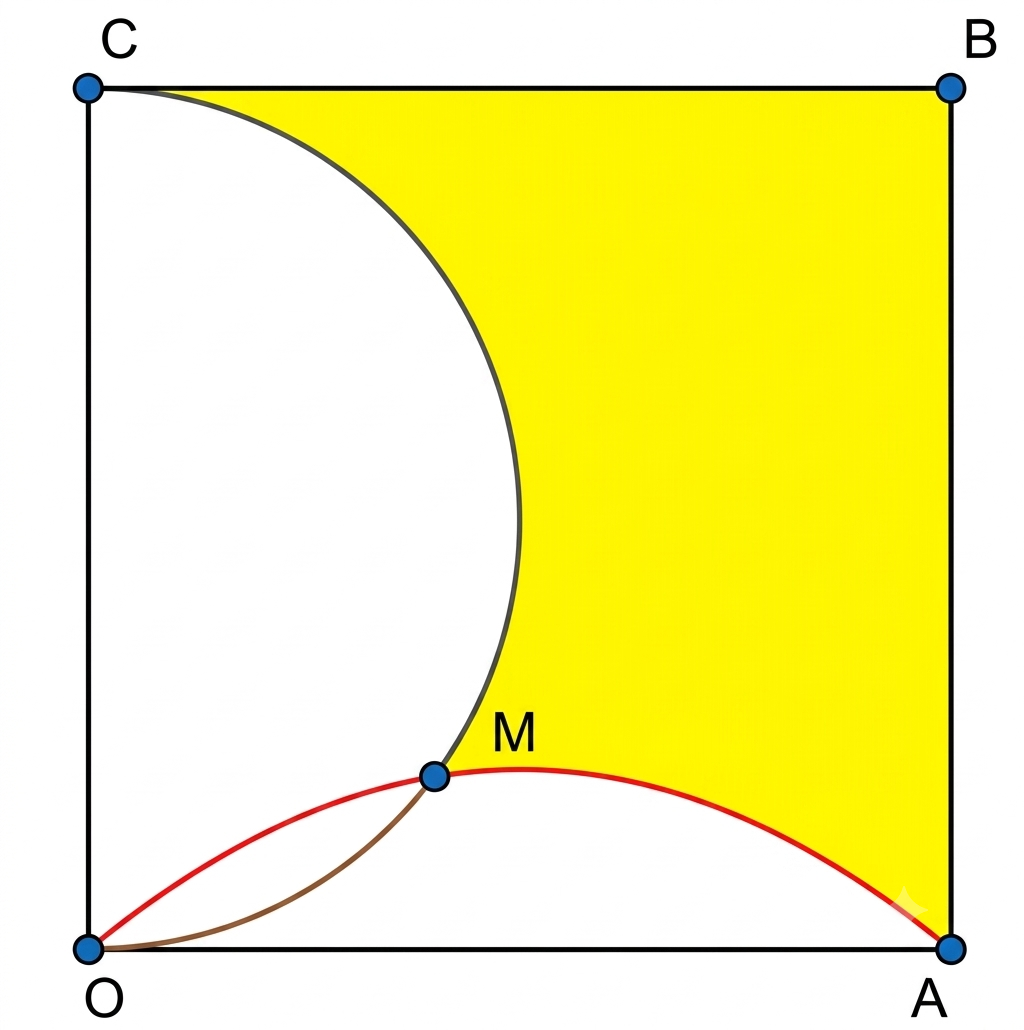
\includegraphics[width=0.4\textwidth]{images/Cau17.png}
\end{figure}
}


\questionShortAnswer{0}{18}{Nghề làm thùng gỗ sồi đựng rượu vang, đặc biệt là chuẩn thùng Barrique của vùng Bordeaux, Pháp, đòi hỏi sự tỉ mỉ và độ chính xác rất cao. Những chiếc thùng này không có dạng hình trụ thẳng đứng mà phình ra ở giữa. Thiết kế này giúp thợ ủ rượu dễ dàng lăn thùng và cặn rượu được gom lại ở phần rốn bụng. Theo tiêu chuẩn sản xuất, đường viền dọc thân thùng cong dạng một cung parabol.
\begin{figure}[H]
    \centering
    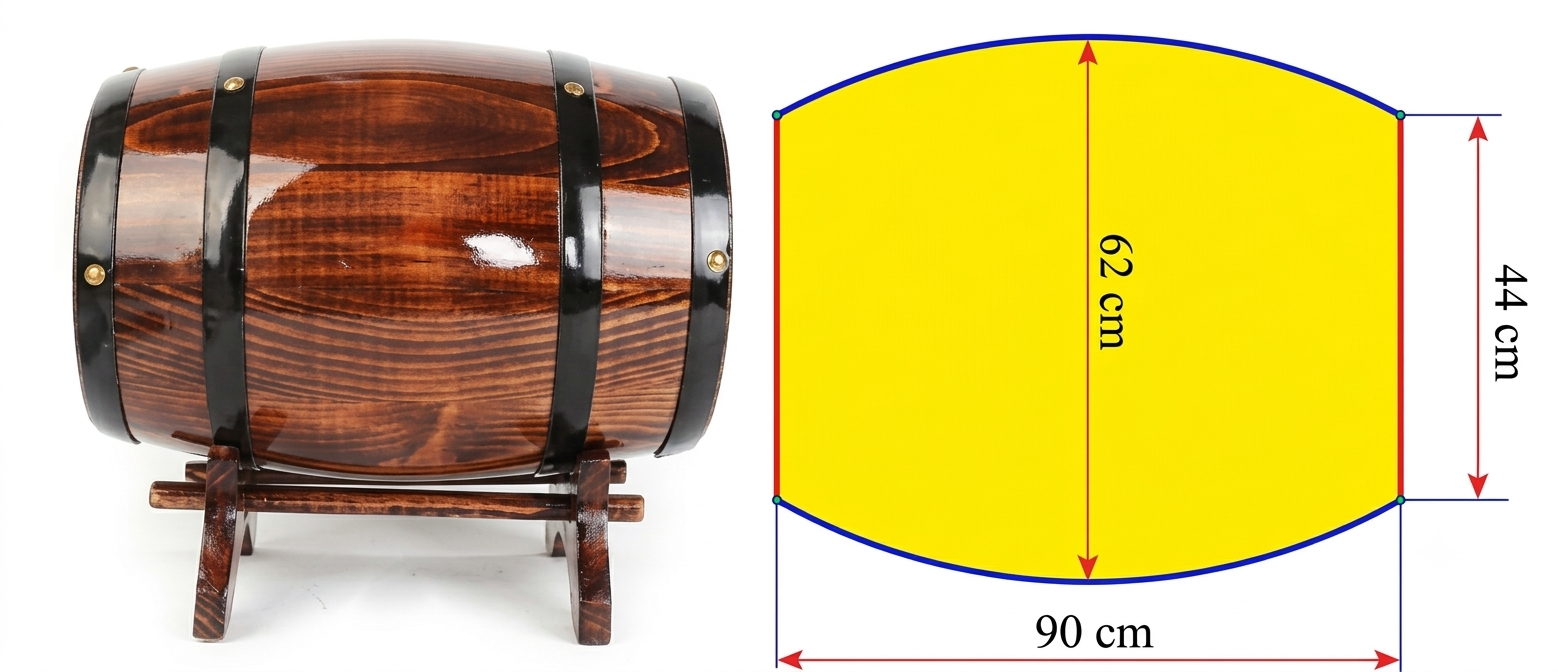
\includegraphics[width=0.7\textwidth]{images/Cau18.png}
\end{figure}
Một xưởng gỗ chuẩn bị xuất xưởng một chiếc thùng có các thông số kỹ thuật được đo đạc cẩn thận. Nhiệm vụ đặt ra là phải tính toán dung tích thực tế của chiếc thùng này để dán nhãn chính xác trước khi đưa vào hầm ủ. Biết rằng thùng rượu vang có chiều cao 90 cm. Đường kính lớn nhất ở phần bụng thùng là 62 cm, trong khi đường kính ở hai mặt đáy của thùng là bằng nhau và bằng 44 cm. Hỏi thể tích của chiếc thùng đó bằng bao nhiêu lít? Làm tròn kết quả đến hàng đơn vị.
}

% --- CÂU 19 ---
\questionShortAnswer{0}{19}{Một công ty hóa chất có một bồn chứa dạng hình nón cụt làm bằng thép, bồn có chiều cao là 4 mét, bán kính đáy dưới là 1 mét và bán kính đáy trên là 3 mét. Giả sử bồn đang trống, người ta bắt đầu bơm một loại dung dịch vào bồn với tốc độ không đổi là 0,5 m\(^3\)/phút. Hỏi sau bao lâu (giây) kể từ khi bắt đầu bơm, mực nước trong bồn đạt độ cao 2 mét?
}

% --- CÂU 20 ---
\questionShortAnswer{0}{20}{Để đảm bảo an toàn khi lưu thông trên đường, các xe ô tô khi dừng đèn đỏ phải cách nhau tối thiểu 1 m. Một ô tô A đang chạy với vận tốc 12 m/s bỗng gặp ô tô B đang dừng đèn đỏ nên ô tô A hãm phanh và chuyển động chậm dần đều với vận tốc được biểu thị bởi công thức \(v_A(t) = 12 - 3t\) (m/s). Hỏi để hai ô tô đạt khoảng cách an toàn khi dừng lại thì ô tô A phải hãm phanh khi cách ô tô B một khoảng ít nhất là bao nhiêu mét?
}

% --- CÂU 21 ---
\questionShortAnswer{0}{21}{Nhà Tít có một bồn chứa nước hình trụ cao 300 cm, đường kính 60 cm. Bồn đầy nước thì bạn Tít vô ý mở van xả. Mực nước hạ với vận tốc \(h'(t) = \dfrac{1}{54}t - \dfrac{10}{3}\) (\(t\) tính bằng phút, \(h'(t)\) cm/phút). Sau 1,5 giờ (tức 90 phút) thì Tít mới phát hiện sự cố. Hỏi lượng nước đã mất là bao nhiêu lít? (làm tròn kết quả đến hàng đơn vị)
\begin{figure}[H]
    \centering
    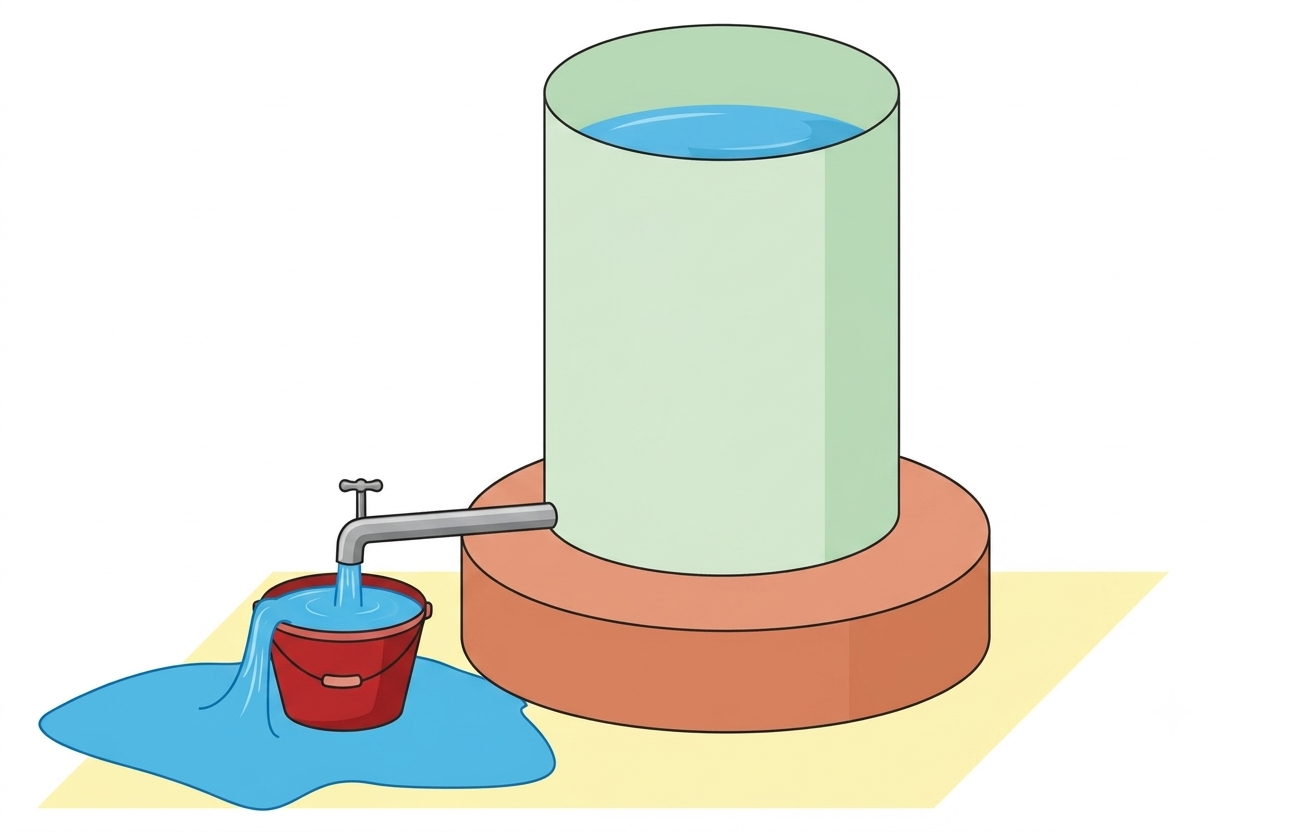
\includegraphics[width=0.4\textwidth]{images/Cau21.png}
\end{figure}
}

% --- CÂU 22 ---
\questionShortAnswer{0}{22}{Trong phim hoạt hình Doraemon, chú mèo máy Doraemon có dùng đến bảo bối Đường hầm Gulliver có tác dụng phóng to hay thu nhỏ hay vật khi đi qua (tham khảo hình vẽ). Bảo bối có hình dạng là như 1 đường hầm, chỉ cần đi vào đường hầm bằng cửa lớn, kết quả thu nhỏ sẽ xuất hiện khi bước ra ở cuối đường hầm và ngược lại. Biết rằng mỗi mặt cắt vuông góc với mặt đáy và song song với mặt phẳng vào hầm có dạng parabol có chiều rộng bằng chiều cao (\(D = h\)) (tham khảo hình vẽ).

\begin{figure}[H]
    \centering
    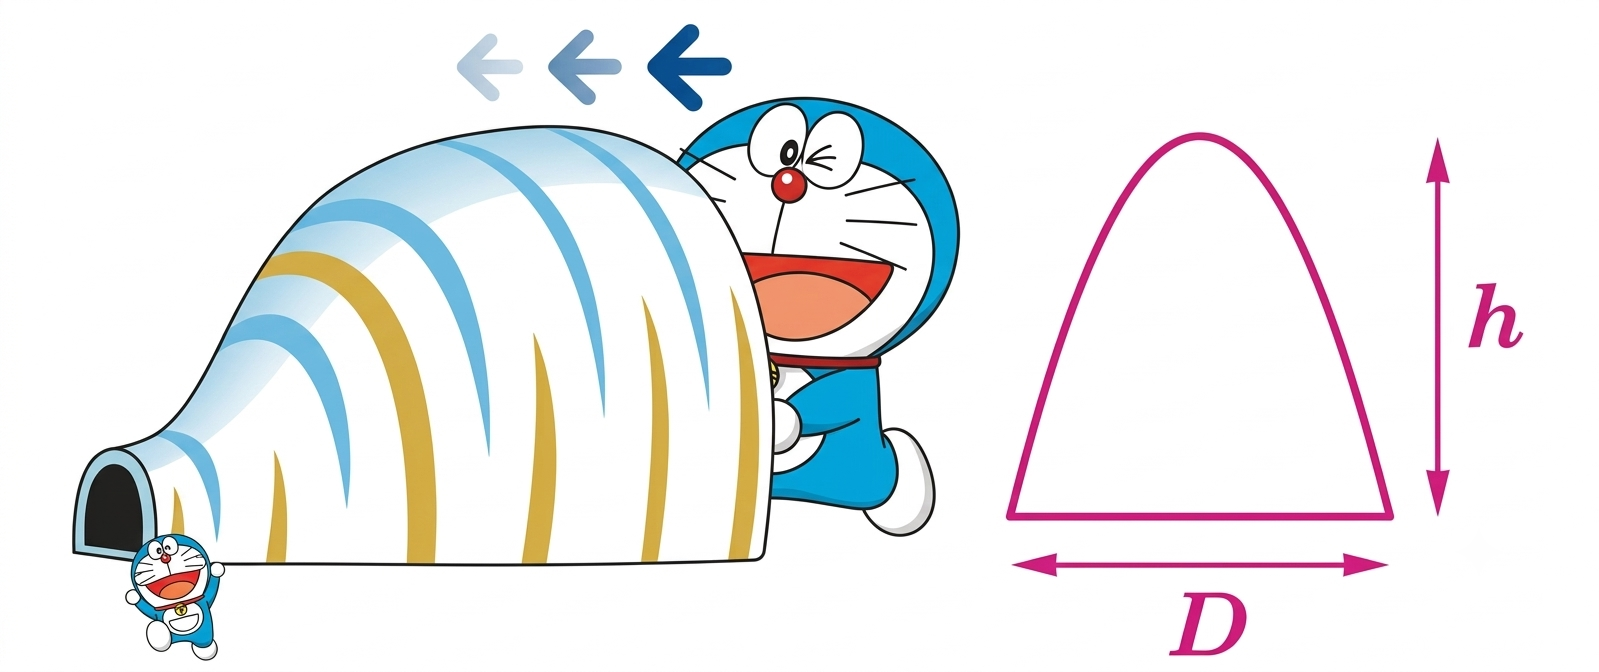
\includegraphics[width=0.6\textwidth]{images/Cau22.png}
\end{figure}

Tất cả các đỉnh parabol mặt cắt có thể mô hình hóa bởi đồ thị hàm số \(y = \dfrac{9}{4000}x^4 - \dfrac{3}{50}x^3 + \dfrac{9}{20}x^2 + \dfrac{5}{2}\), \(0 \leq x \leq 10\), với mặt cắt tại \(x = 0\) là cửa nhỏ của đường hầm, mặt cắt tại \(x = 10\) là cửa lớn của đường hầm, đơn vị trên hệ trục tọa độ dài 1 dm. Tính thể tích của đường hầm (đơn vị dm\(^3\), kết quả làm tròn đến hàng đơn vị).
}

\end{document}
%I: 1A, 2A, 3B, 4A, 5A, 6C, 7C, 8C, 9B, 10A, 11B, 12D
%II: 13SSDD, 14DSDS, 15DSDS, 16SSSS
%III: 17:197 ,18:224, 19:29.3, 20:25, 21:636, 22:374
